\documentclass{standalone}
\usepackage{tikz,ctex}
\usepackage{tikz-3dplot} % 2-1
\usepackage{unicode-math} % 2-5,4-1,4-2
\setmathfont{Fira Math Regular}
\setmainfont{Fira Sans}
\definecolor{background}{RGB}{239, 239, 239} % 4-5,6-2,6-5
\begin{document}
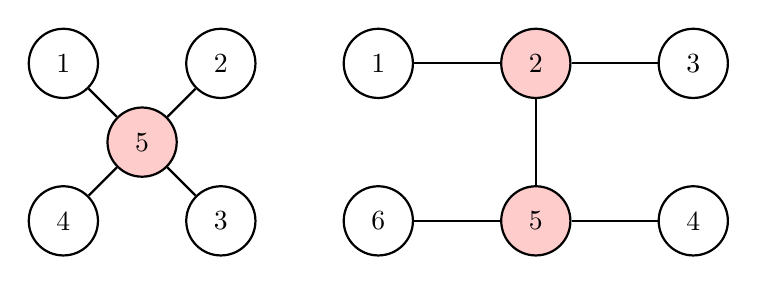
\begin{tikzpicture}
\foreach \x/\y/\a[count=\i] in{0/2/1,2/2/2,2/0/3,0/0/4,4/2/1,8/2/3,8/0/4,4/0/6}{
    \node[circle,minimum size=25pt,thick,draw] (\i) at(\x,\y) {\a};}
\foreach \x/\y/\a[count=\i] in{1/1/5,6/2/2,6/0/5}{
    \node[circle,minimum size=25pt,thick,fill=red!20,draw] (1\i) at(\x,\y) {\a};}
\foreach \u/\v in{1/11,2/11,3/11,4/11,5/12,6/12,7/13,8/13,12/13}{
    \draw[thick] (\u)--(\v);}
\end{tikzpicture}
\end{document}